\chapter{Design Engineering Process} 
Summarize the breakdown of the des eng process here ??.

\section{Research Aims and Goals}

\subsection{Context and Rationale}
This project addresses fabric waste in garment manufacturing by aiming to make zero-waste pattern making more accessible and inclusive. It seeks to resolve the lack of parameterisation methods for zero-waste patterns and the inability of current patterns to provide a good fit for diverse body types. Custom sizing for individuals enhances the garment's value to the wearer, but introducing more fit can lead to increased cut loss. Therefore, the project aims to present methods to recoup cut loss through creative reuse for increased garment utility. The project leverages virtual draping tools to provide visual representations before users commit to production.

\subsection{Scope}
This project targets the smaller-scale operations that can more readily adopt innovative and sustainable practices. It is not concerned with the mass production but rather the creation of a single garment for an individual. Integration of fabric properties and cost analysis are not considered. 

The aim is to create a framework enabling bespoke towards zero-waste pattern creation for both virtual modelling and physical production. The framework provides analytics on fabric use efficiency to enable informed decisions.  

This project selected one existing zero-waste pattern to parameterise and is not concerned with developing a new pattern design. The project prioritises fit around the bodice over arms. Physical testing in a workshop study is used for evaluating the parameterisation method on fit. Theoretical analysis on a publicly available dataset is used for evaluating the parameterisation on fabric efficiency and cut loss metrics.
 
The author is not trained in fashion practice but applies design engineering methods to introduce novelty. Python is used for parameterisation, pattern file generation, and efficiency analysis. CLO 3D is used for virtual draping.

\subsection{Goals}
Key goals of the project include:
\begin{itemize}
    \item Develop a method that successfully takes in measurements and outputs a parameterised pattern for the garment.
    \item Calculate the ideal fabric bolt width for a given pattern's dimensions.
    \item Compute fabric efficiency and cut loss metrics based on user preferences for informed decision-making.
    \item Provide mitigation techniques to fit the pattern on available fabric bolt widths.
    \item Define and implement a strategy that repurposes cut loss to enhance the garment's utility and aesthetic appeal.
    \item Generate pattern files to visualise the garment on an avatar.
\end{itemize}

\section{Methodology}

\subsection{tail0r Pipeline}

\subsection{Pattern Selection}
The chosen garment for this study is Helmersson's short-sleeved collared shirt with a back pleat and front button closure (Figure \ref{fig:bh shirt sketch}) from her book \textit{Zero Waste Patterns: 20 Projects to Sew Your Own Wardrobe}. It's a ``one-size garment where the total body circumference [of the garment] is determined by the width of fabric'' used, forcing zero-waste. As a result, it's inherently loose-fitting and oversized, presenting a unique challenge in balancing zero-waste principles with a more tailored fit. She designates it as skill level 3 out of 5, being suitable for confident beginners. The garment was chosen for its relative simplicity in construction, symmetry of its pattern (Figure \ref{fig:bh shirt pattern}), and the challenge it presents in parameterising for a better fit.
\begin{figure} [H]
    \centering
    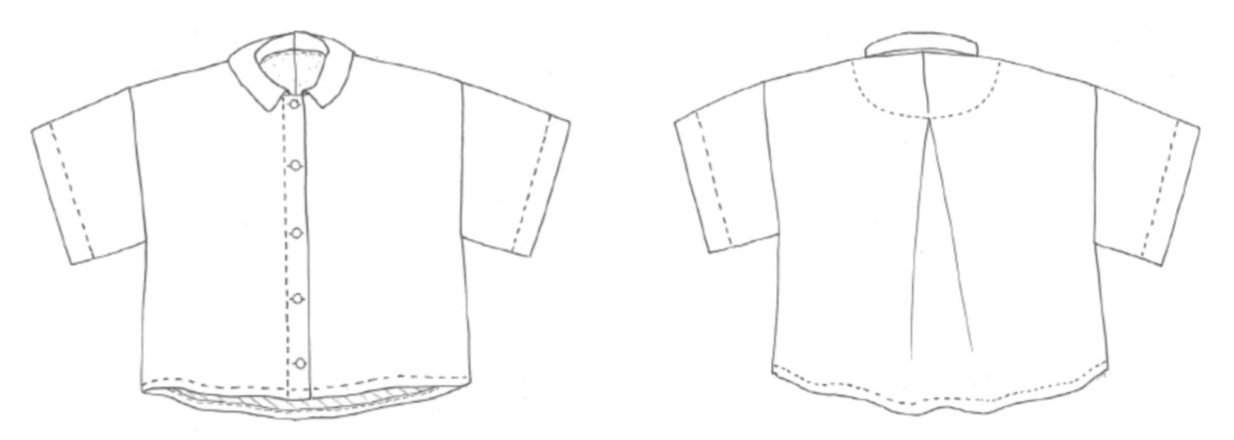
\includegraphics[width = \textwidth]{Images/finishedgarmentsilhoutte.png}
    \caption{Helmersson's Shirt sketch}
    \copyright {Birgitta Helmersson} % this prints the caption below the figure
    \label{fig:bh shirt sketch}
\end{figure}
\begin{figure} [H]
    \centering
    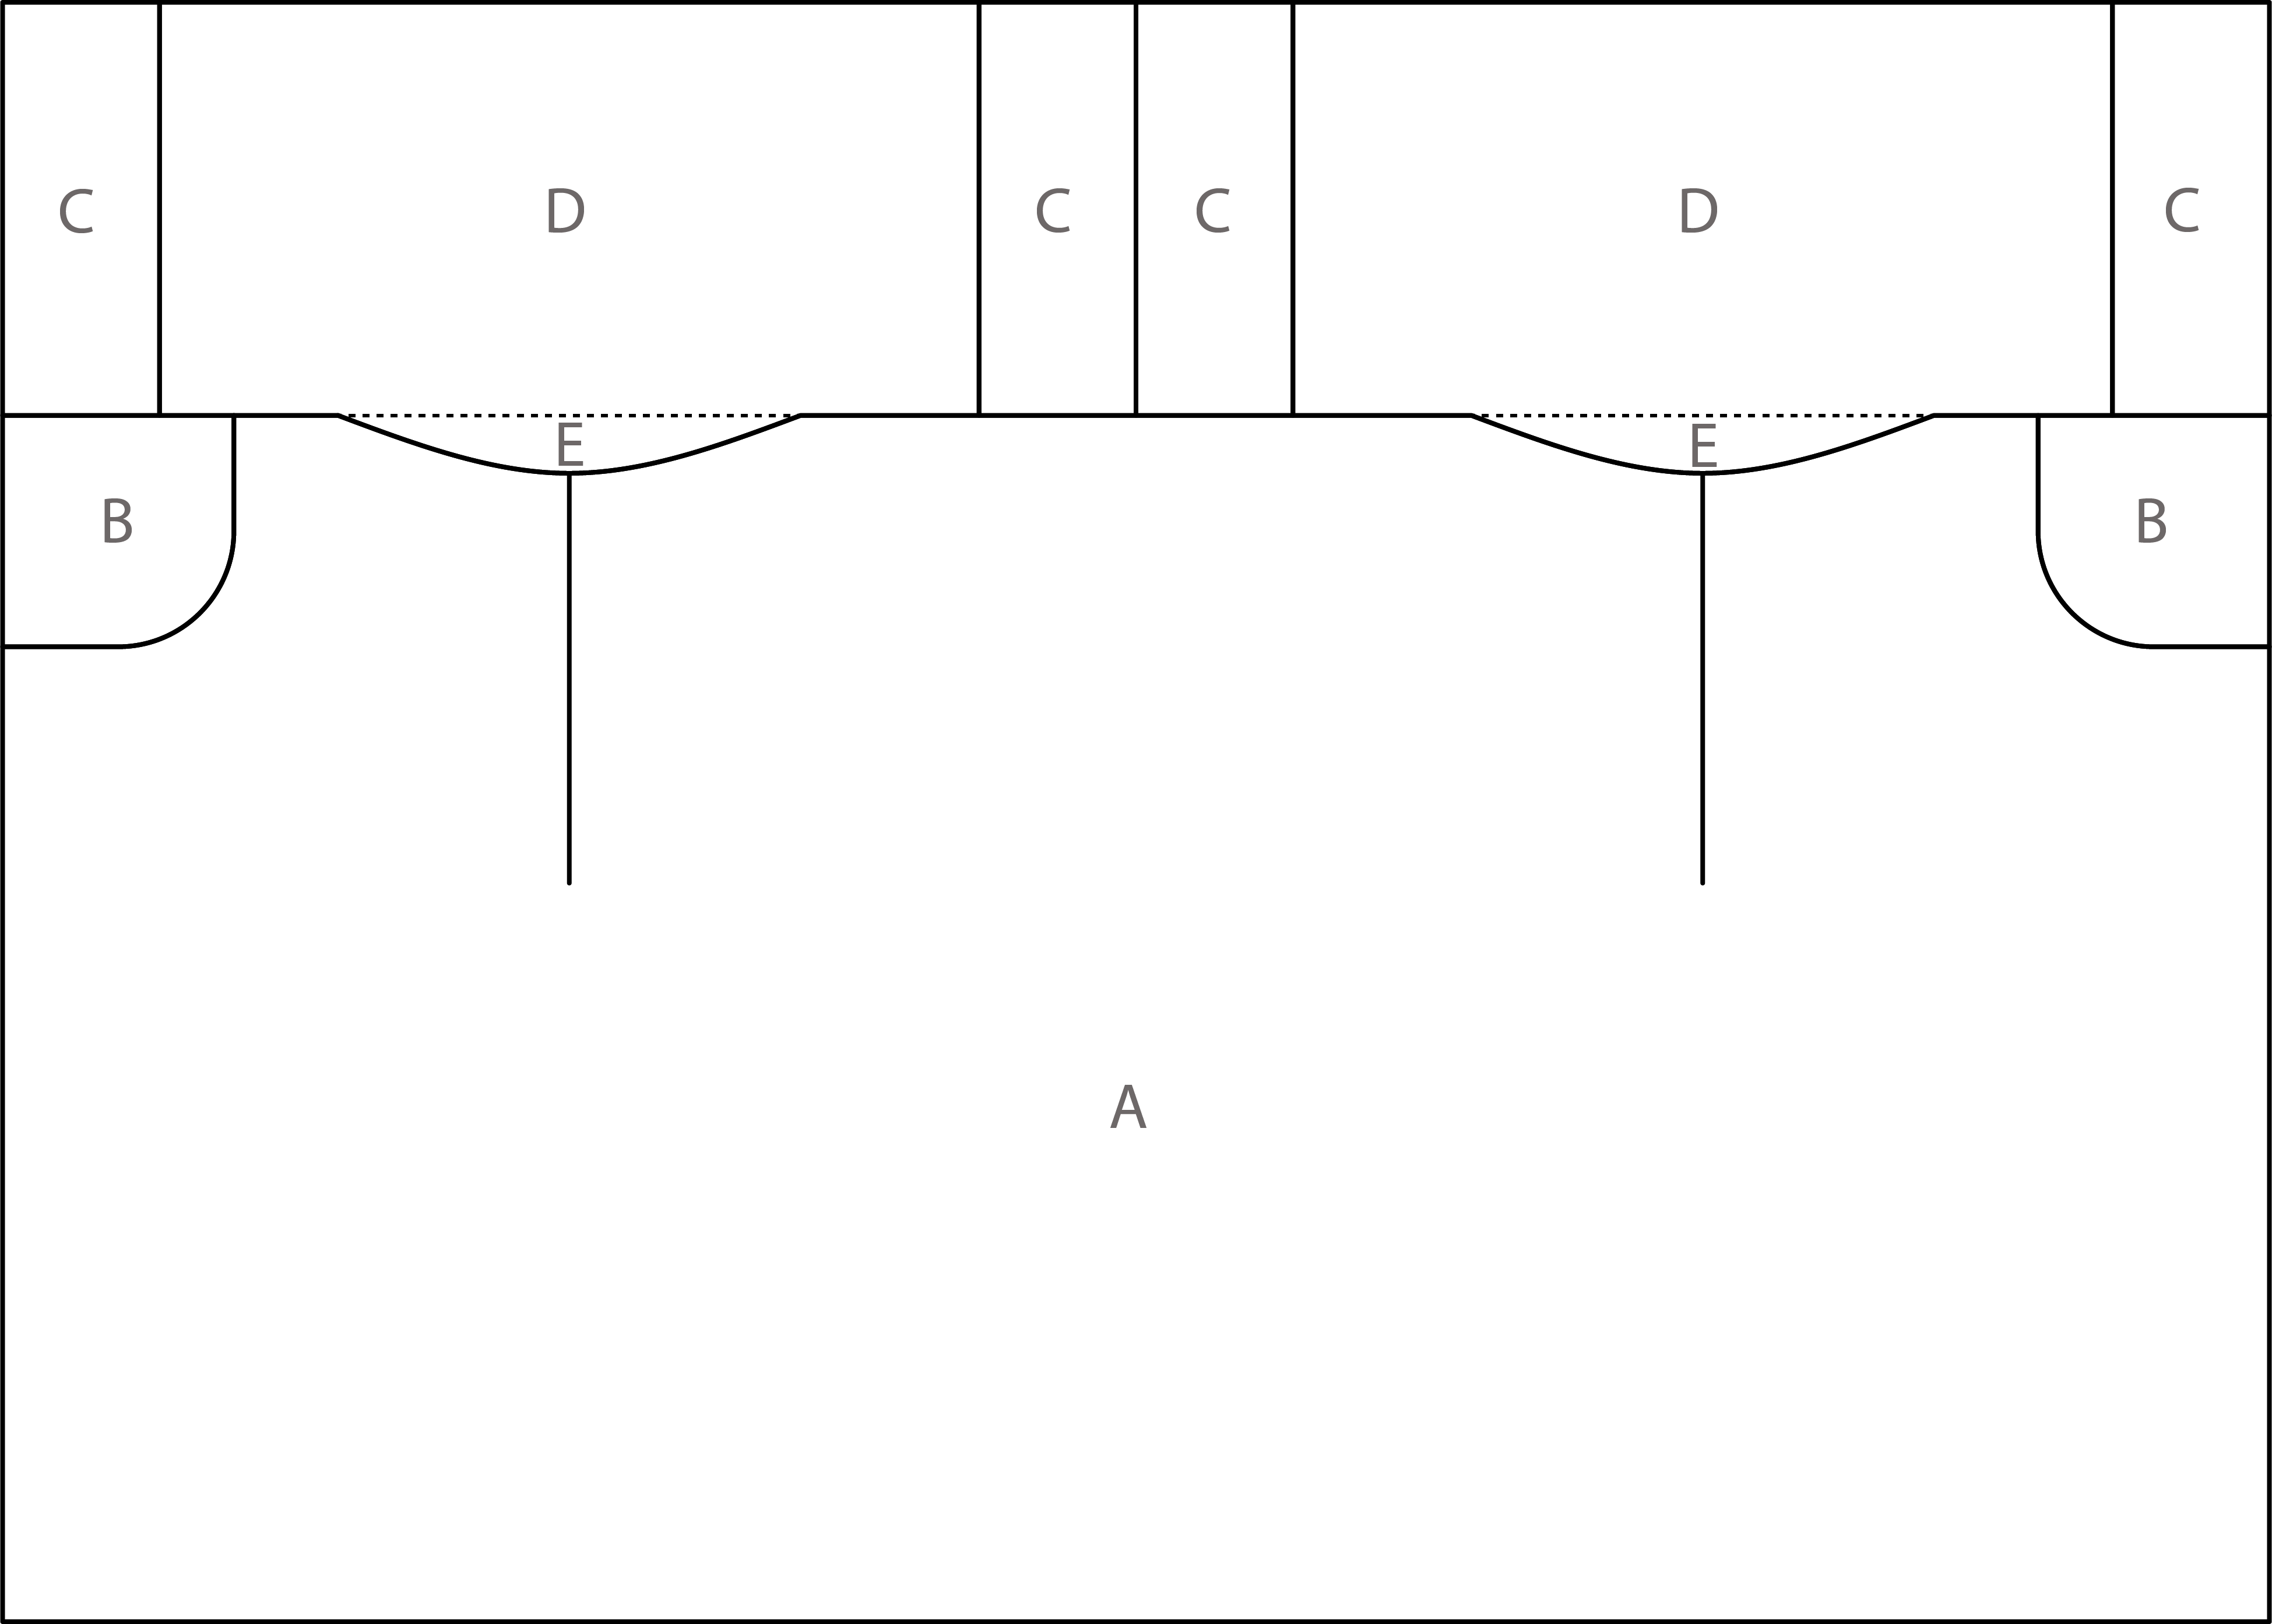
\includegraphics[width = 0.75\textwidth]{Images/originalpattern_whole.png} 
    \caption{Shirt block pattern}
    \label{fig:bh shirt pattern}
\end{figure}
\begin{itemize}
    \item \textbf{A} Front/back body piece
    \item \textbf{B} Back neck facing template
    \item \textbf{C} Collar pieces
    \item \textbf{D} Sleeve pieces
    \item \textbf{E} Sleevehead curve template
\end{itemize}
Helmersson's method does not require large paper patterns; instead, designs are drawn directly onto the fabric and cut. For constant pieces, she provides small printable templates, maintaining fixed sizes for B, C, and E. Her sizing chart (Figure \ref{fig:bh size chart}) includes about 25 of ease, combining both wering and design ease. This ease is applied generally, not to individual areas. The chart only considers fabric widths within a 20 cm range and bases sizing only on chest/bust and hip measurements, with fabric with being 31 cm greater than the largest max circumference. This includes 25 cm of ease and 6 cm seam allowance, values used for parameterisation.
\begin{figure} [H]
    \centering
    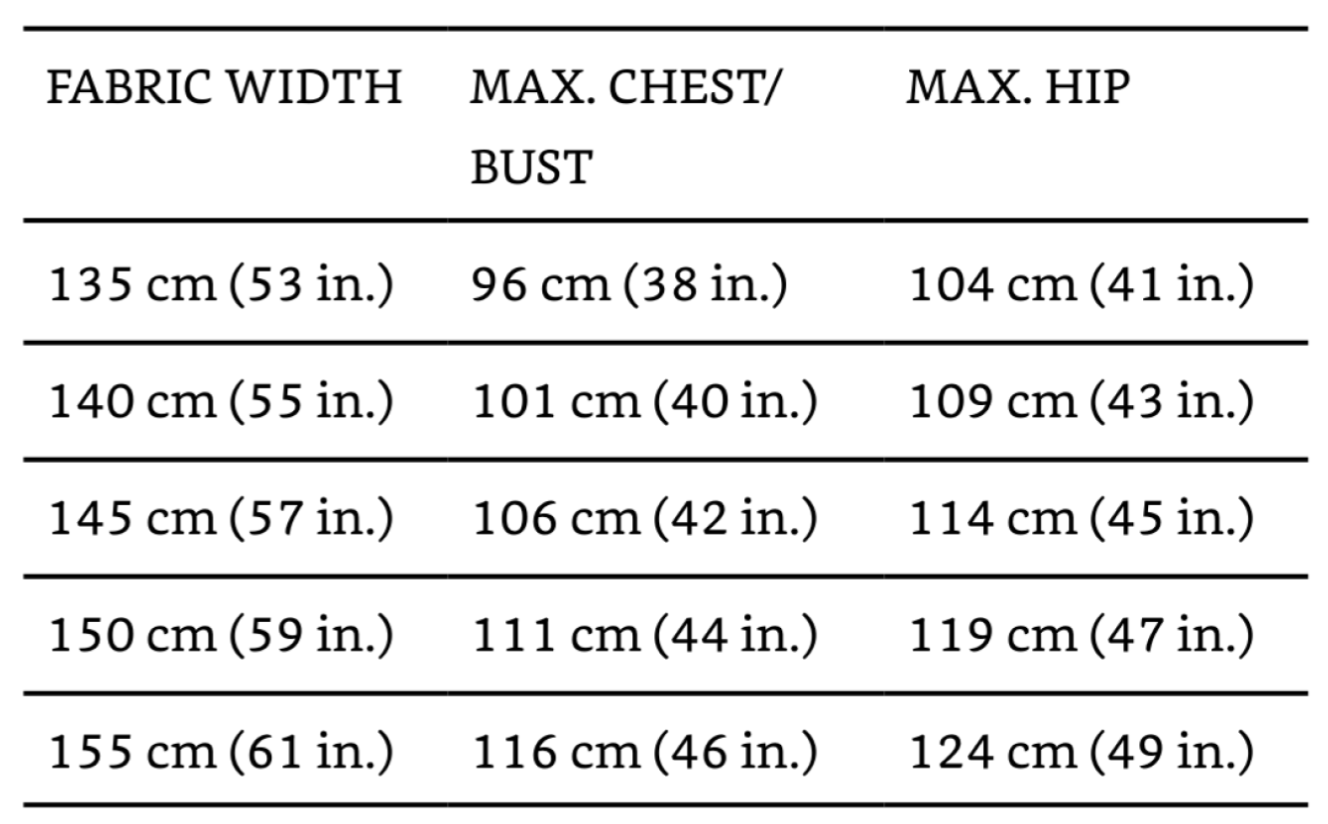
\includegraphics[width = 0.5\textwidth]{Images/BH size chart.png} 
    \caption{Helmersson's Shirt sizing chart}
    \copyright {Birgitta Helmersson}
    \label{fig:bh size chart}
\end{figure}
Notions (bindings, buttons, iron on interfacings, etc.) are not considered. These are components of the final garment not sourced from the original rectangle cut from the fabric bolt, therefore, are not part of the waste analysis.

%%%%%%%%%%%%%%%%%%%%%%%%
% PATTERN PARAMETERISATION
%%%%%%%%%%%%%%%%%%%%%%%%

\subsection{Pattern Parameterisation}
Now that the original garment type is understood, we can dissect the pattern into individual segments for parameterisation.
\begin{figure} [H] 
    \centering 
    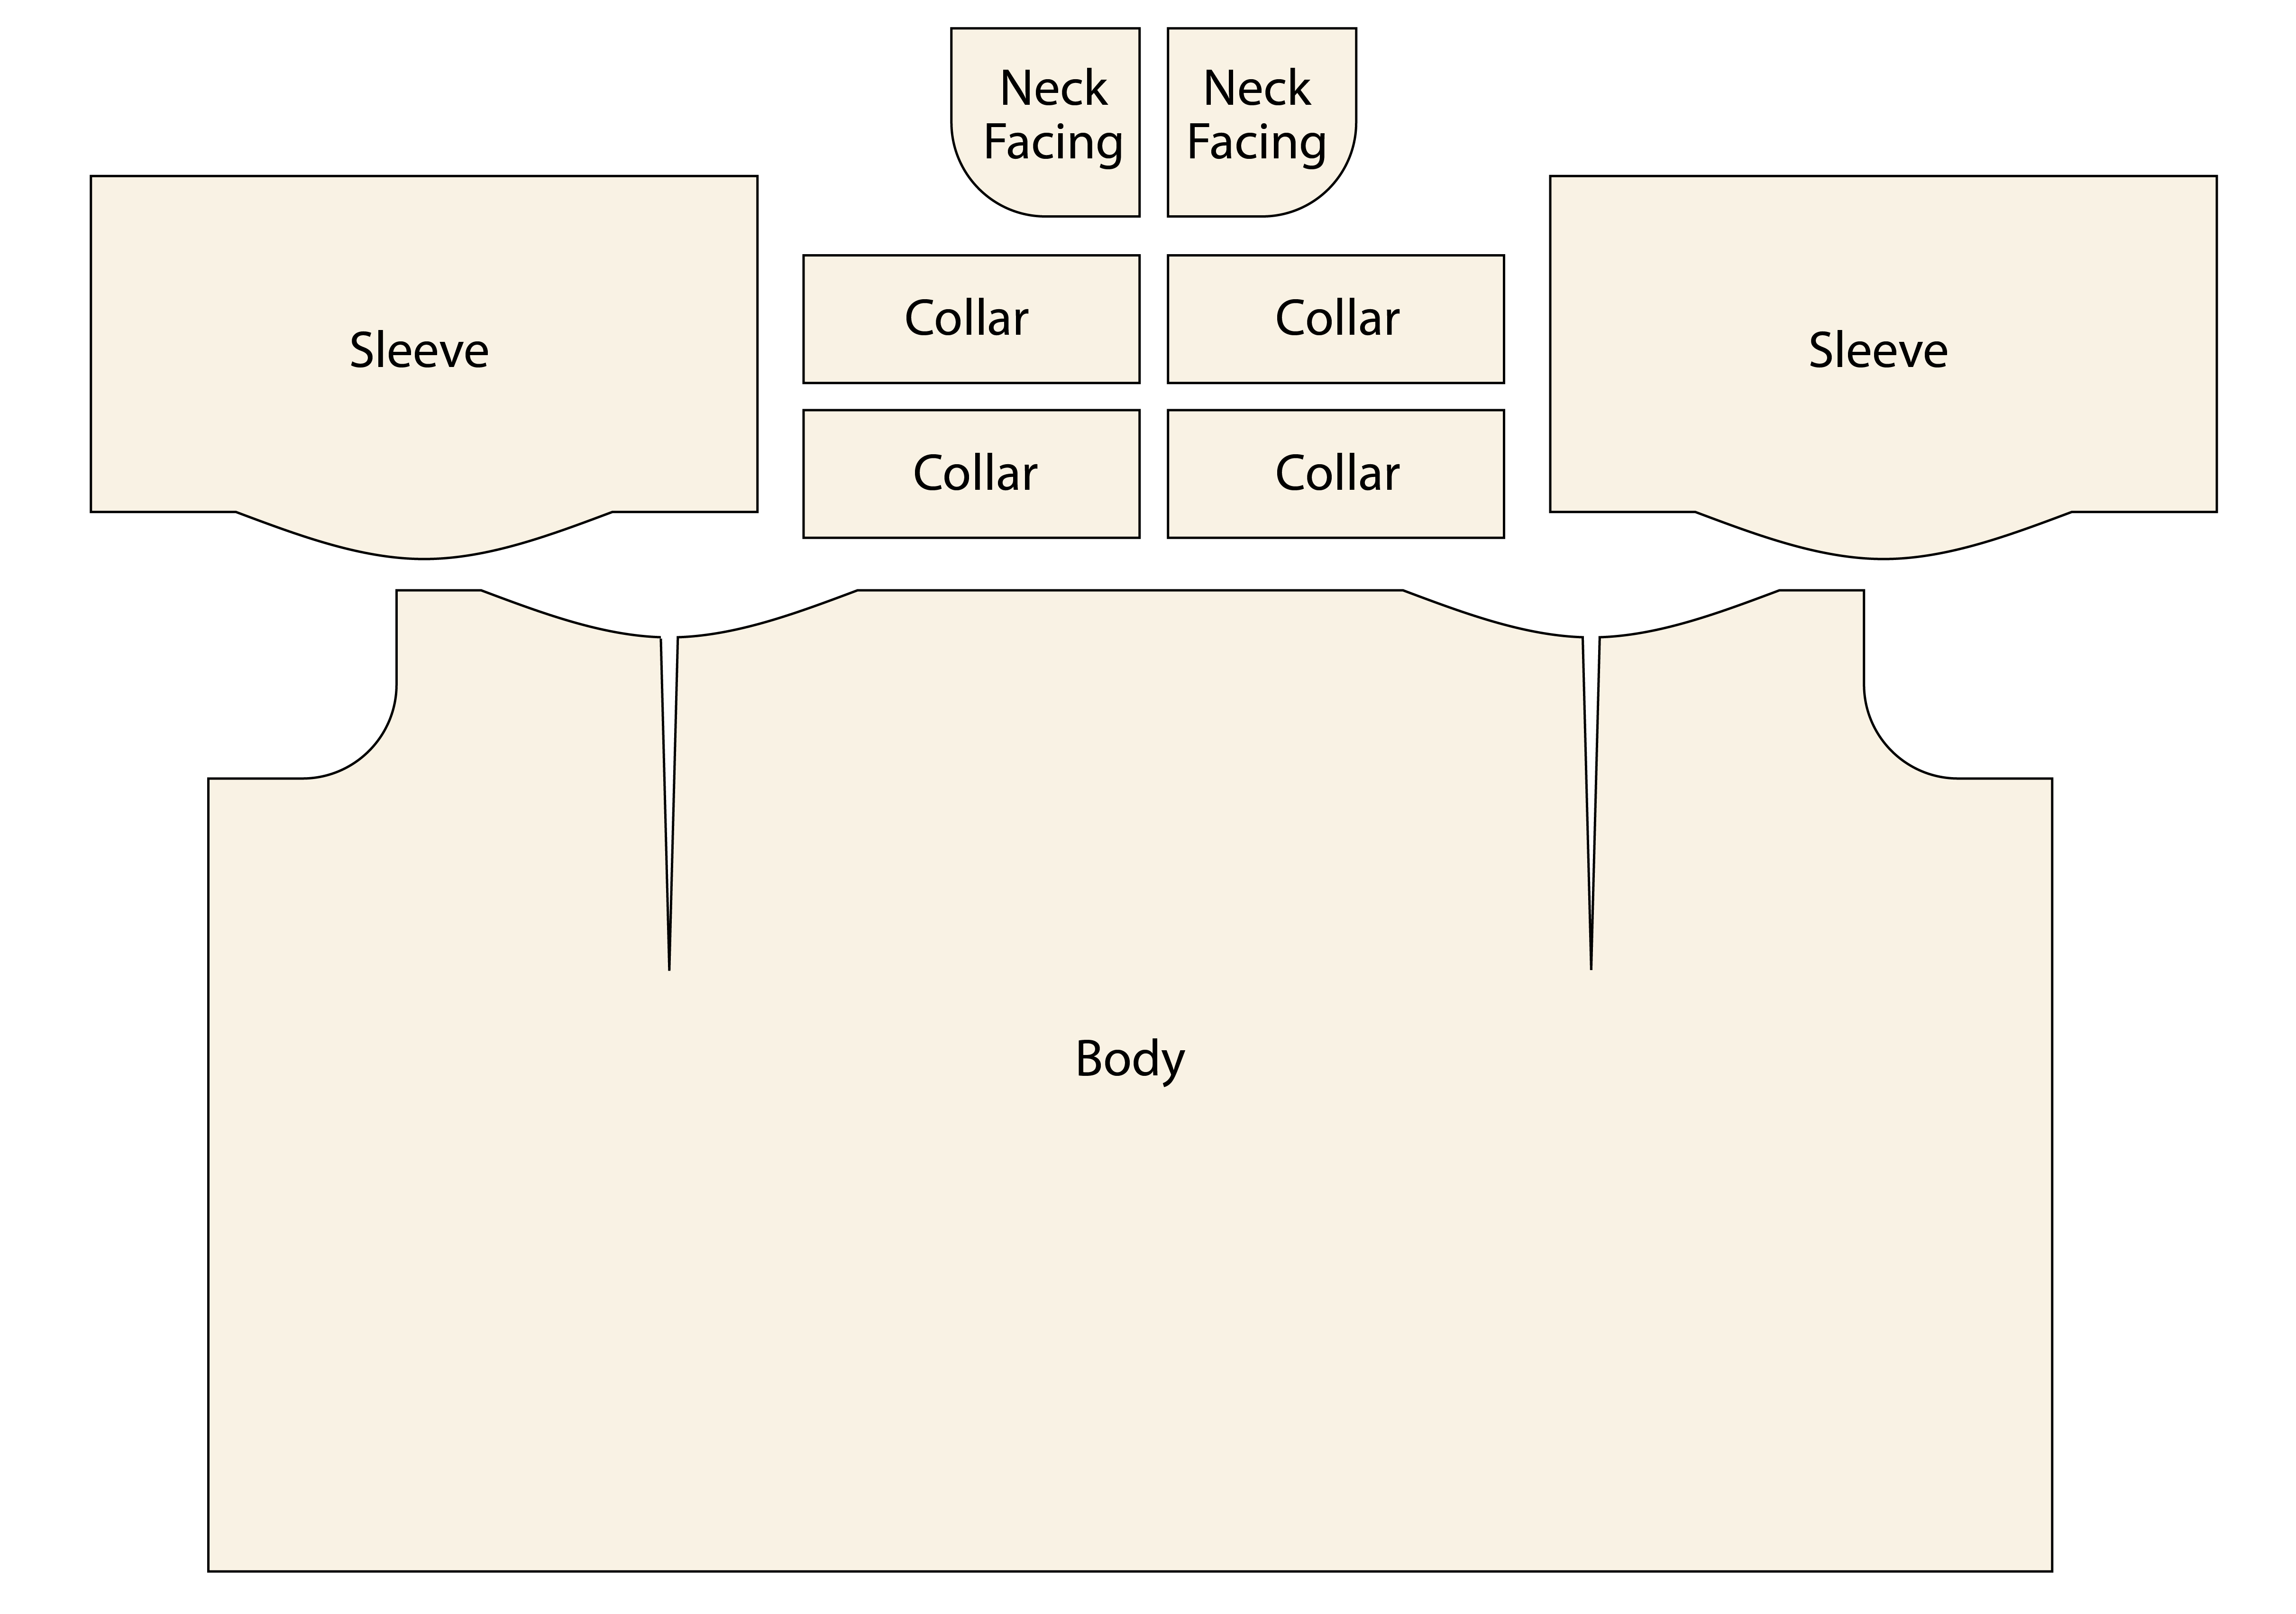
\includegraphics[width = \textwidth]{Images/originalpattern_pieces.png} 
    \caption{Shirt block pattern pieces}
\end{figure}
There are a total of nine (1x body, 2x neck facing, 4x collar, 2x sleeve) pieces that make up the block. Note that D and E combine to form the sleeve piece. There are no side seams on the shirt as there is just a single body piece, not a separate front and back.

\begin{table} [H] % this tells the compiler that a table environment is starting
    \centering % this puts it in the horizontal centre of the page
    %\rowcolors{1}{}{Gray} % this sets up the alternating grey/white background
    \begin{tabular}{p{2cm}|p{5cm}} % this sets up the tabular environment ant states the width of the columns, you could use an equation here using the \textwidth, but i have no experience with this. 
    
        %the following lines populate the table with data. They follow the pattern
        % item & item & item & item \\
        % where the ampersand denotes a vertical line, and the double slash, a new line.
        \textbf{Shortform} & \textbf{Parameter}\\
        \hline % this produces a horizontal line, this could be used elsewhere in the table
        pw& pattern width\\
        ph& pattern height\\
        cw& collar piece width\\
        ch& collar piece height\\
        bw& neck facing width\\
        bh& neck facing height\\
        sd& sleevehead curve depth\\
        sr& sleevehead curve radius\\
        al& armhole length
        \end{tabular}
    \caption{Pattern Parameters Table}
\end{table}
\begin{figure} [H] % opens the figure environment. the '[H]' forces the image to be Here
    \centering % puts the image in the horizontal centre of the page
    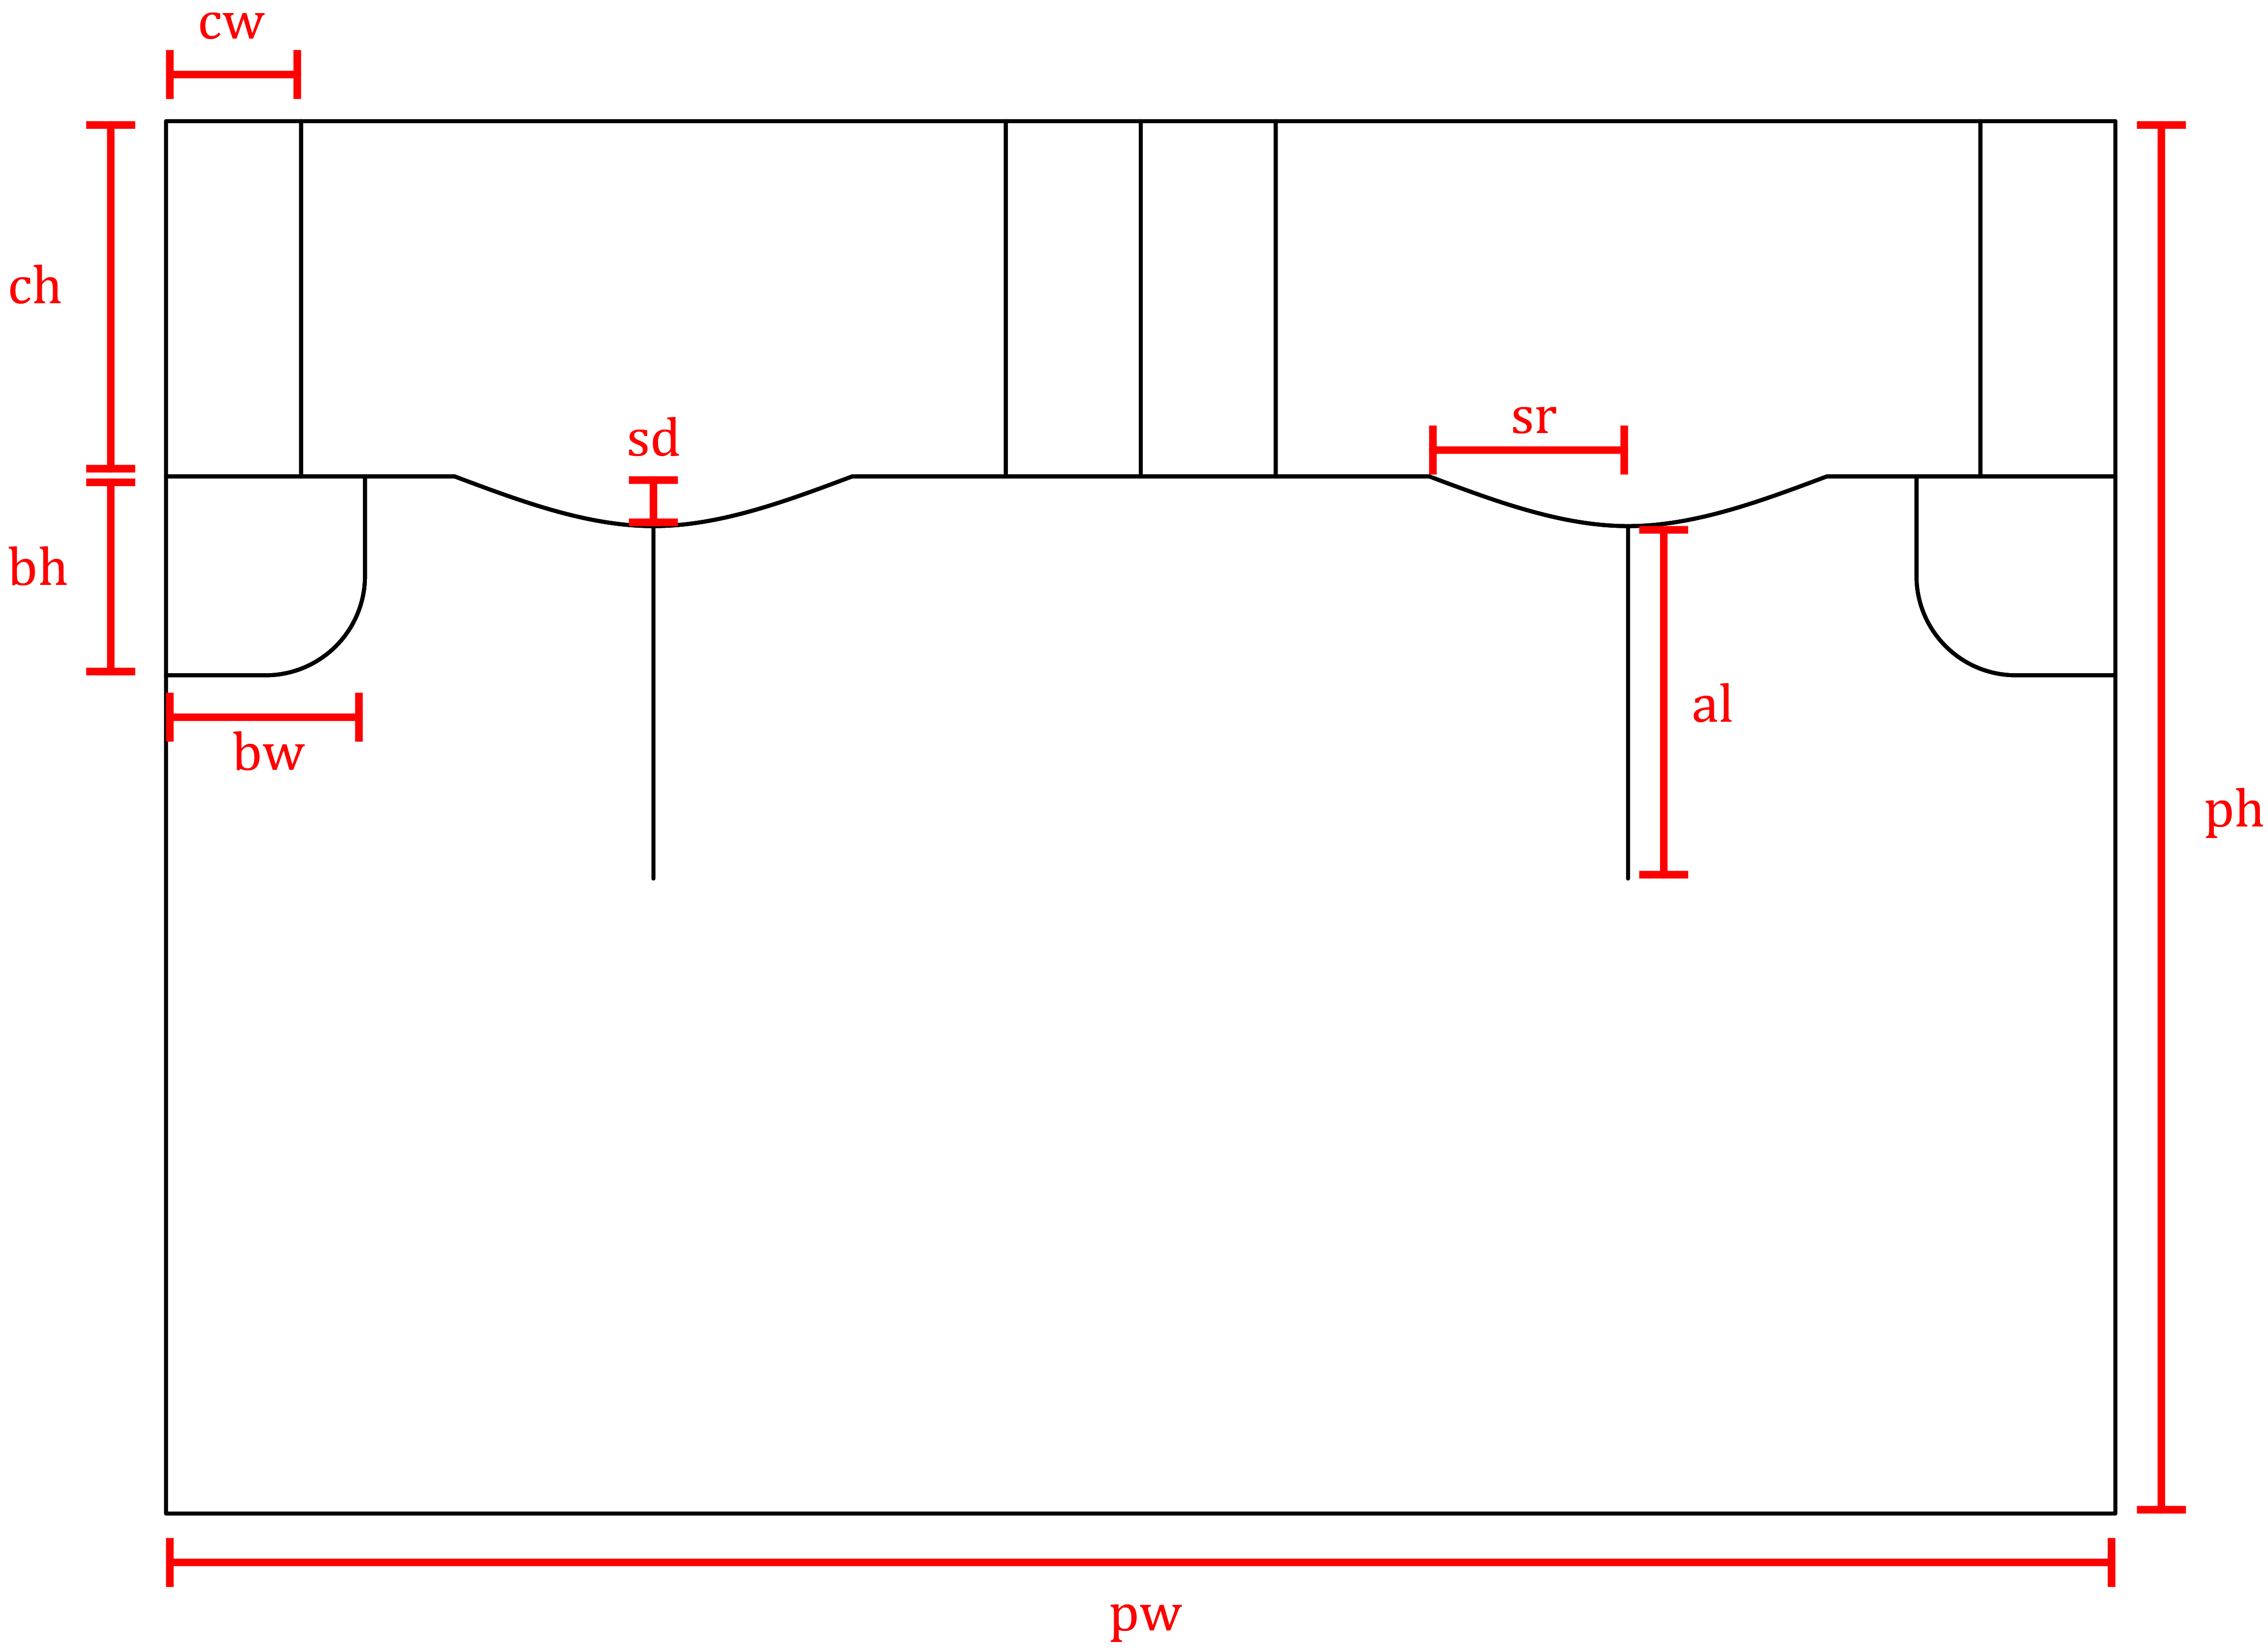
\includegraphics[width = \textwidth]{Images/pattern params.png} %this tells latex what graphics to include. I put my images in an 'Images' folder to aid file management, hence the Images/ before the file name. the width bit before allows you to alter the width of the image. It is also possible to use scale as well as using equations with the textwidth to make it say half the text width.
    \caption{Pattern Parameters Diagram}
\end{figure}

The process for parameterising was based on traditional measurements professionals use for a tailored shirt. How these measurements can translate into algorithm for the pattern parameterisation was investigated.

By looking at the pattern, we quickly realise that scaling one dimension has an effect in multiple pieces. For example, increasing the pattern width will also enlarge the sleeve pieces. Therefore, it requires some nuance and compromise to be able to scale pieces effectively while still keeping the rectangular nature of the overall pattern. We are primarily concerned with calculating the pattern width and pattern height as these define the pattern at large. We are less focused on the definition of each piece's dimensions at input because some of these factors will be deduced by the pattern width and pattern height along with the layout of the pieces given the fabric bolt used to make the garment.

The fit around the bodice is the primary factor to be customised. Given this, the process starts by defining what will be kept constant. The collar piece is kept constant inline with Helmersson's dimension suggestions with collar piece width of 9.5 cm and collar piece height of 25 cm. It becomes clear that a segment is shared between the collar piece (C) and the sleeve piece (D). Collar piece height corresponds to the sleeve length measured from the shoulder point to the sleeve end(barring any hemming for now). The first relationship between pattern and finished garment discovered is that the sleeve length equals the collar piece height, 25 cm in this case.

The placement of the notches used to determine the finished pleat size and the button placket are also kept constant for everyone. For now, the general ease of the garment will also be constant with Helmersson's suggestion of 25 cm. Results from the workshop may reveal that general ease should be dependent on some measurement factor.

The collar piece height also influences the overall pattern height. The height of the body piece (A) plus the collar piece height equals the total pattern height. From the center back linein the pattern, it is evident that the height of the body piece can be related to the shirt length measured from the center back base of the neck to the finished hem at the bottom. Shirt length is a personal choice and not a strict body measurement based input. The garment will employ a standard shirt 2.5 cm hem at the bottom for a clean finished. This hem allowance must be considered as it will come from the original fabric piece in maintaining zero waste design.
\begin{equation}
    \mathrm{pattern\ height} = \mathrm{desired\ shirt\ length} + \mathrm{collar\ piece\ height} + \mathrm{hem\ allowance}
    \label{eq:pattern height}
\end{equation}

with shortform and constants,

$ph = desired shirt length + ch + hem allowance$

if shirt length is 65 cm 

$ph = desired shirt length + 25 + 2.5$

The parameterisation assumes the pattern with will be equal to the largest circumference of the bodice plus the general ease and sew allowance for the body. We still intend to keep the aesthetic of the garment while provide fit to extend garment utility in terms of more wear time/uses.
\begin{equation}
    \mathrm{pattern\ width} = \mathrm{largest\ bodice\ circumference} + \mathrm{general\ ease} + \mathrm{sew\ allowance}
    \label{eq:pattern width}
\end{equation}

with short and constants,

$pw = largest bodice circumference + 25 + 6$

From the pattern, it is clear that scaling pattern width had an effect on the sleeve pieces. The collar piece widths (cw) are kept constant. By looking at the top border of the pattern, we see that pattern width also equals four collar piece widths plus two (one for each sleeve piece) top edge segments of the of the sleeve.

pw = 4*cw + 2*(sleeve top edge)

therefore

sleeve top edge = (pw - 4*cw) / 2

The sleeve top edge represented the sleeve circumference. Therefore, scaling up the pattern width will also scale up the sleeve circumference i.e. larger bodies will have baggier sleeves.
The armhole length (al) is equal to half of the sleeve top edge. This is because when the sleeve is sewed it needs to fit in the armhole with is formed when cutting the armhole length at the middle of the sleevehead curve and sewing the shoulder seams.

al = (pw - 4*cw) / 4

What is left is deciding how to scale the template sizes. Starting from her pattern as inspiration, we are simplifying the pattern even further to use simpler shapes when constructing these templates. Based on her size chart we are identifying an "ideal" largest circumference range for this pattern based on her chart and using her expertise as a fashion designer. This ideal range for the pattern then is 95cm to 125cm. We will use this ideal range to determine if a person gets the standard template size. People below this range will get slight smaller template size and people above this range will get bigger template size. Helmersson claims that beyond 25 cm of these measurements then the pattern might not be suited for you, we are aiming to make it more inclusive and account for other custom sizes with out parameterisation. It is important to recognize that proportions of human body do not scale 1 to 1. People can still have short height and gurthy necks for example.

For the standard neck facing template (B) size, We use square and circle inscribed in that square for the simple shape. Remember that these pieces help form the button placket, front neck line, and the overall pieces for the back neck facing. The facing piece height and width equal each other at 14 cm.

bw = bh = 14 cm

The facing piece curve horizontal line segment and facing piece curve vertical line segment are equal to each other and also equal to half of the facing piece width.

bx = by = (bw/2) = 14/2 = 7 cm

This 7 cm will also be the radius of the circle used to form the curve corner of the piece. So it is a quarter circle with radius of 7 cm forming and its end joins with the ends of horizontal and vertical line segments of the piece.

For the sleevehead curve template (E), an approximated and simplified verson of BH's template is using a sleevehead curve radius of 14cm and and sleevehead curve depth of 3.5cm. Notice that the sleevehead curve radius and facing piece width/height are the same. We keep this same relationship for deciding the other two template sizes.

For below 95cm largest circ, we decrease the template size of facing piece width and height as 12 cm, sleevehead curve radius at 12 cm, and sleevehead curve depth at 3.0cm.
For above 125cm largest circ, we increase the template size of facing piece width and height as 16 cm, sleevehead curve radius at 16 cm, and sleevehead curve depth at 4.0cm.
So it is a ±2 cm for the B5 piece width/height and sleevehead curve radius, and a ±0.5cm for the sleevehead curve depth.

The sleevehead curve depth influences the point where the sleeve attaches to the body at the shoulder point. We need to consider appropriate scaling of neck facing and sleevehead curve template because it affects the shoulder seam lengths. If these were always kept constant, it is possible that for smaller pattern widths it will eat into the top shoulder seams length and not fit the person because it is too small. This is a point we need to test for and do in the workshop. We will test if we are being too aggressive with this or not and if there are any not as obvious consequences.

The shapes were simplified not only to make recreating the pattern easier and more standardized but also for ease of use when constructing the pattern in DXF file format. The simple shapes help to streamline and ensure lines were meet at shared points, essential for ensuring the closed shape. 

%%%%%%%%%%%%%%%%%%%%%%%%
% FRAMEWORK OUTPUTS
%%%%%%%%%%%%%%%%%%%%%%%%

\subsection{tail0r Outputs}
The program creates the following outputs:
\begin{enumerate}
    \item A choice of patterns based on user's fit, style, and waste choices.
    \item Fabric usage efficiency metrics using ideal and given bolt widths for pattern choice.
    \item Embellishment strategies and applications for both.
    \item The DXF file that can be loaded into the CLO application for virtual draping and visual fit cues.
    \item The PDF file with return pattern measurements and annotated pattern image with dimensions that allows user to draw pattern on fabric and cut it out pattern.
\end{enumerate}

\subsubsection{DXF Pattern File}
The DXF file format is a standard of digital garment patterns. This format can be imported into many different pattern and 3D fashion applications including CLO 3D. The ‘ezdxf’ Python library was used for creating the DXF files of the pattern. Line, spline, lightweight polyline, and arc primitives were built into base functions to map out the geometry. The accompanying ‘ezdxf viewer’ was used for output verification. Three examples of customised DXF test patterns are shown below.

\begin{figure} [H] % opens the figure environment. the '[H]' forces the image to be Here
    \centering % puts the image in the horizontal centre of the page
    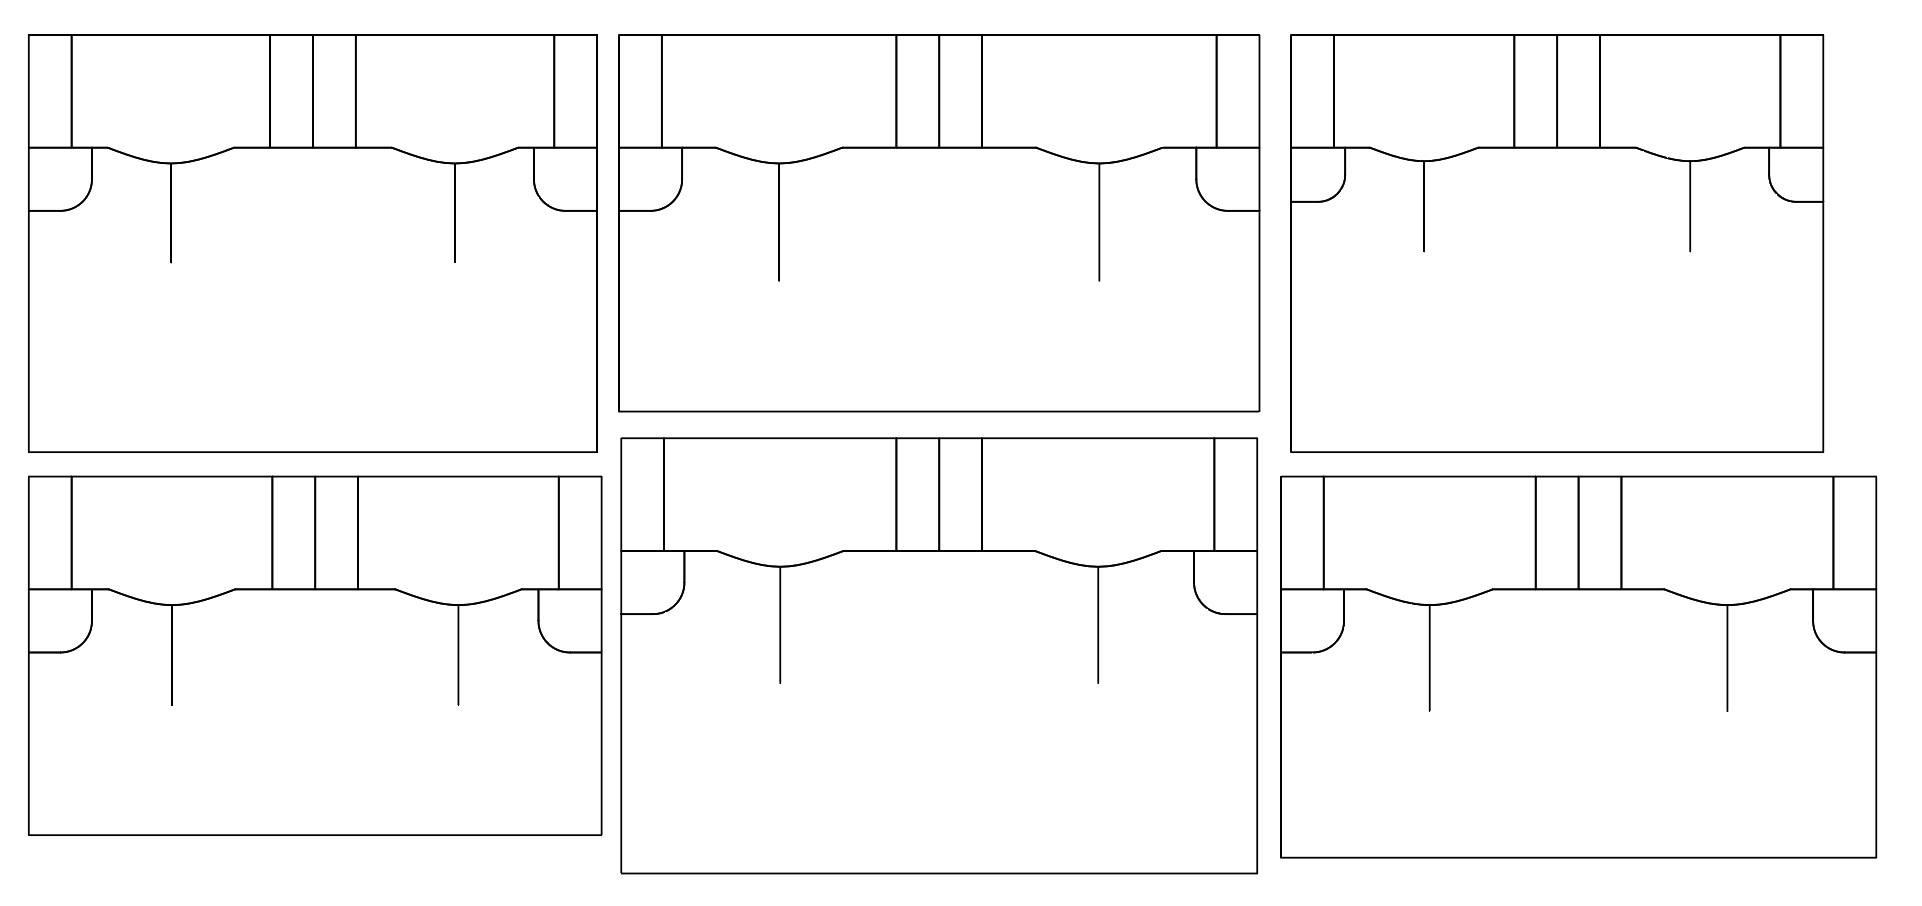
\includegraphics[width = \textwidth]{Images/example dxfs.png} %this tells latex what graphics to include. I put my images in an 'Images' folder to aid file management, hence the Images/ before the file name. the width bit before allows you to alter the width of the image. It is also possible to use scale as well as using equations with the textwidth to make it say half the text width.
    \caption{Examples of DXF pattern outputs in ezdxf viewer}
\end{figure}


CLO 3D has some added requirements. Each pattern piece created via DXF needs to be a closed shape for it to render properly in CLO 3D. Pieces that shared borders need to have their own representation of the shared segment and thus had to be redrawn as needed for the number of pieces they help define. This was achieved by defining layers for each piece type within the document modelspace.

\begin{figure} [H] % opens the figure environment. the '[H]' forces the image to be Here
    \centering % puts the image in the horizontal centre of the page
    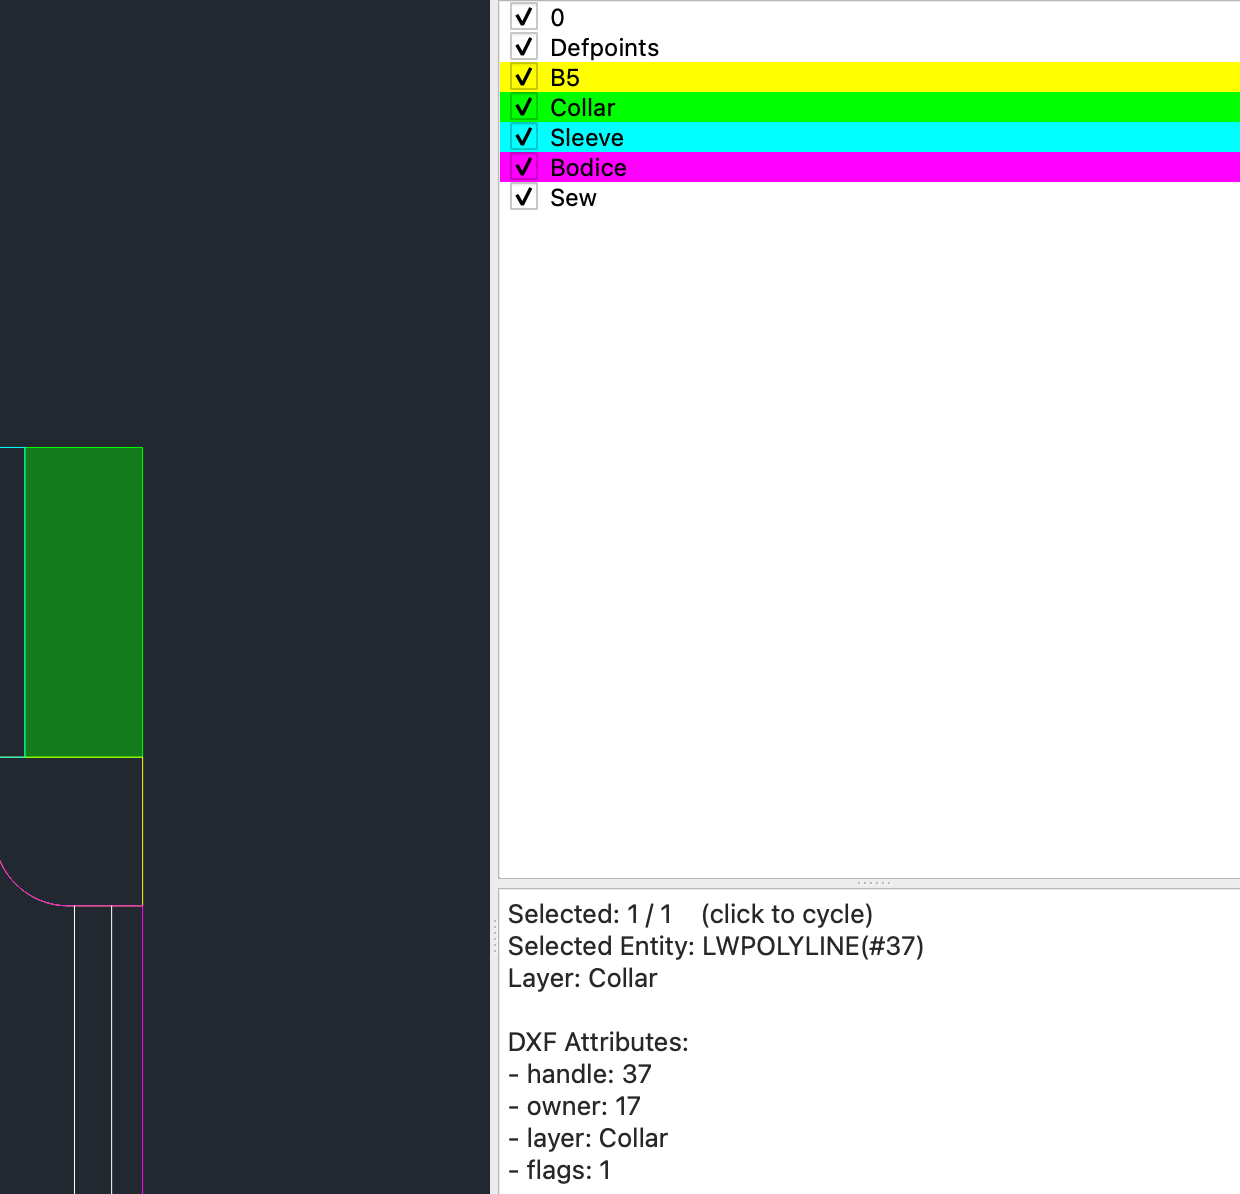
\includegraphics[width = 0.4\textwidth]{Images/dxf viewer.png} %this tells latex what graphics to include. I put my images in an 'Images' folder to aid file management, hence the Images/ before the file name. the width bit before allows you to alter the width of the image. It is also possible to use scale as well as using equations with the textwidth to make it say half the text width.
    \caption{Layer toggle feature in ezdxf viewer}
\end{figure}

Sometimes, these segments had to be manipulated in Adobe Illustrator to get the shapes to close and be usable in CLO 3D. Defining layers easily allowed for paths to be joined with out affecting other pieces. A future enhancement would be to get this to work directly out of Python and ezdxf settings. This process does generate a DXF file suitable for CLO 3D, and once the appropriate sewing properties are defined and pieces are positioned, the garment gets draped onto an avatar. This can then be rendered and shown to the end user as a base visual indication of fit and style.

\subsubsection{PDF Pattern File}
Along with the DXF file, a PDF file is also provided including annotated dimensions of the pattern. It provides all the information needed for measuring, drawing the pattern pieces, and cutting out pieces from the fabric. Labels and dimensions are also presented. This information along with the sewing instructions is what is needed for the user to make the garment themselves. The PDF pattern is made by plotting with matplotlib. An example PDF output is shown below.
\begin{figure} [H]
    \centering
    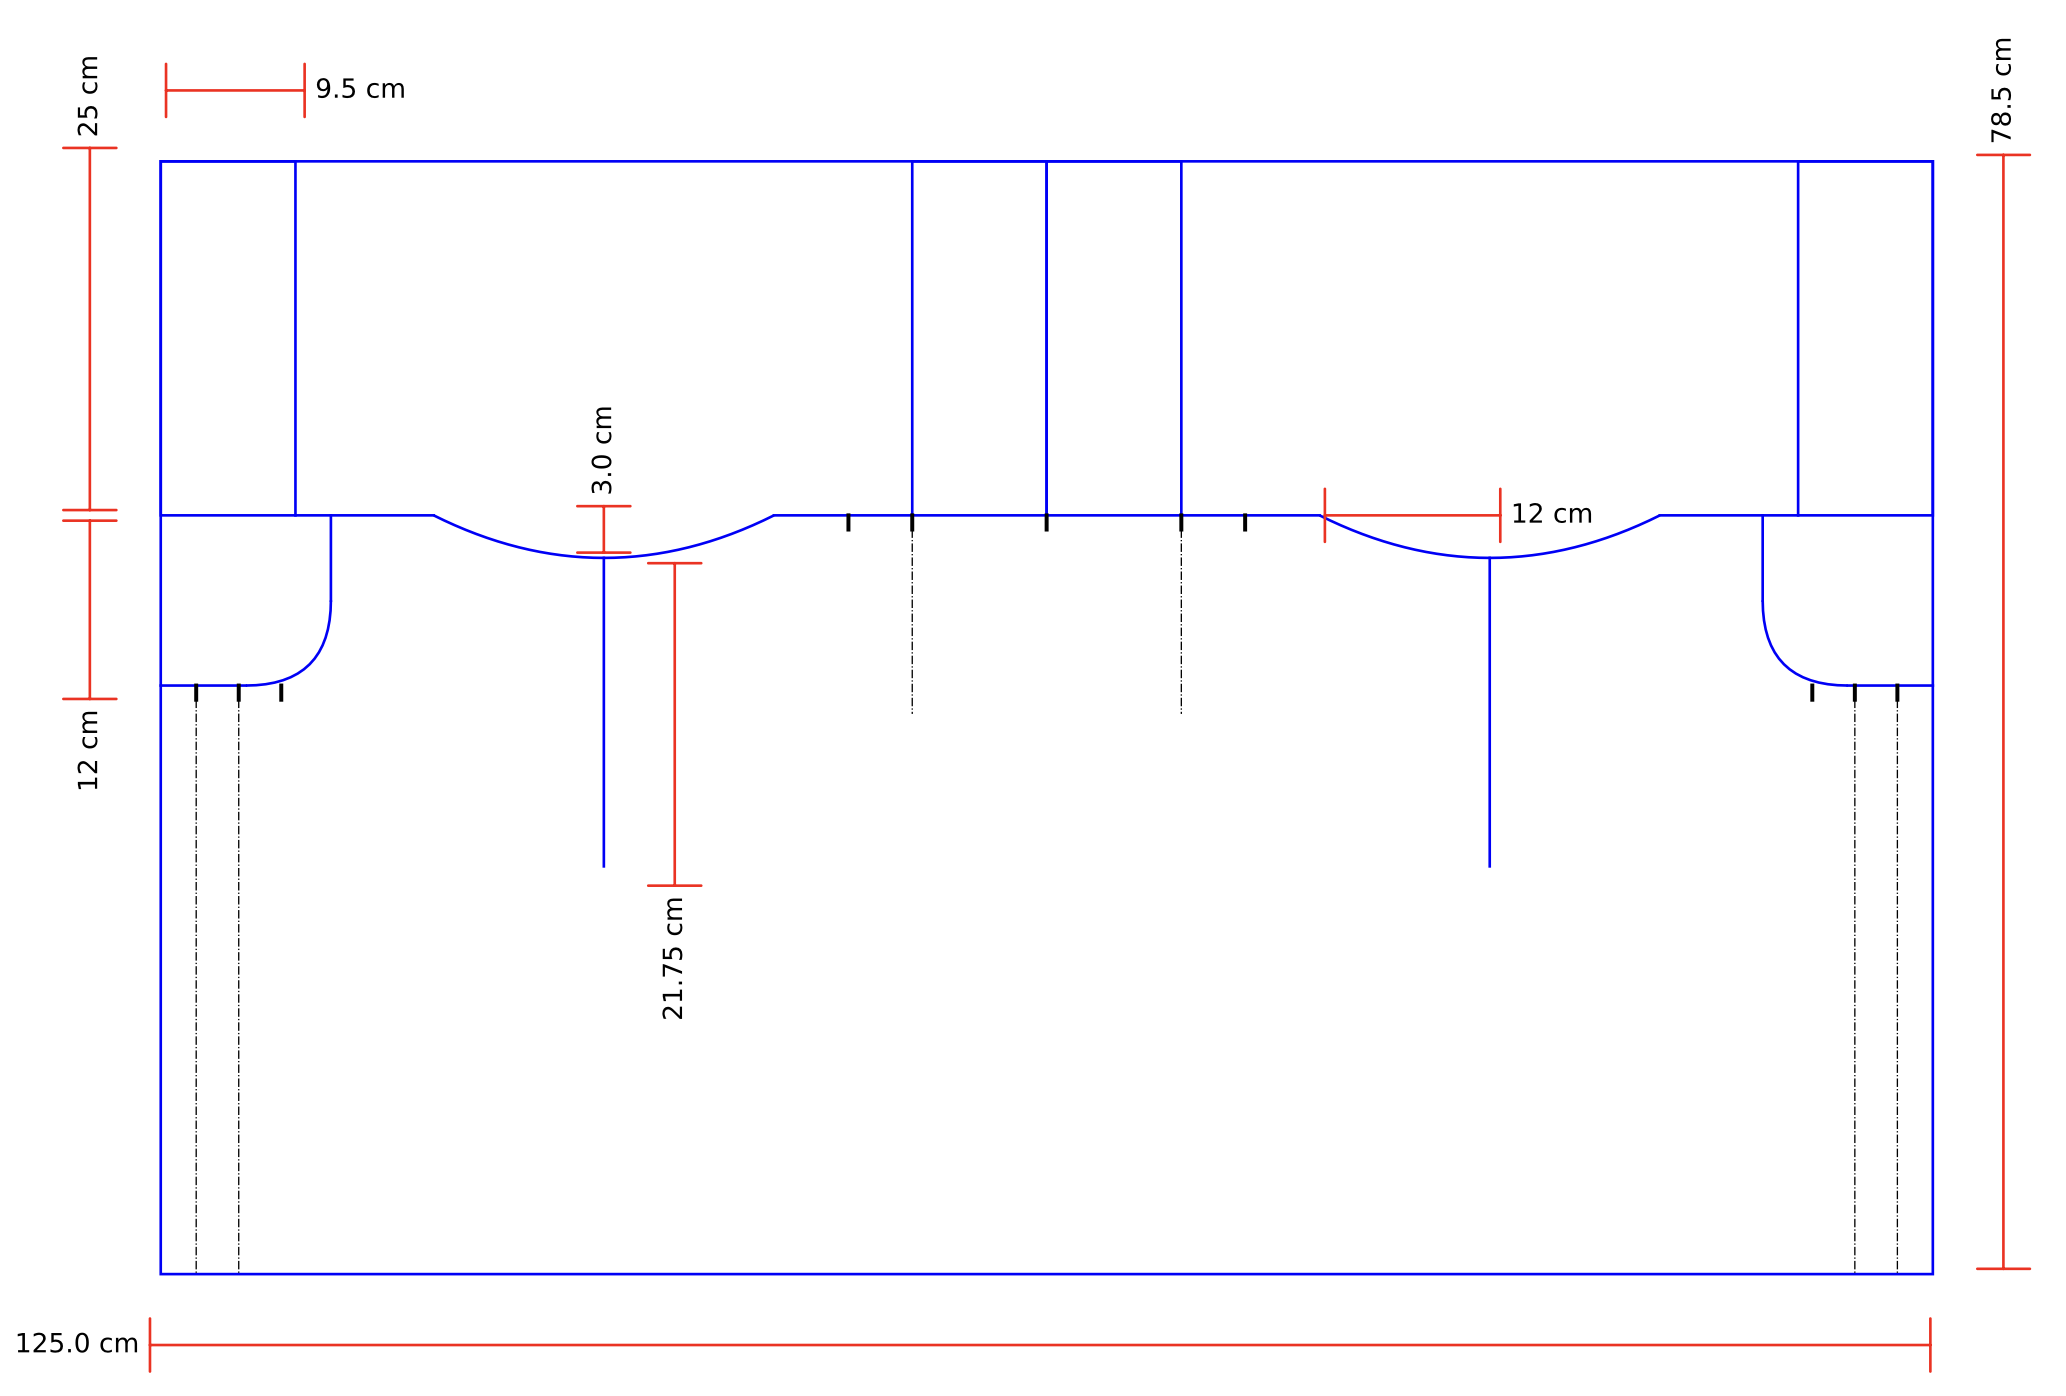
\includegraphics[width = \textwidth]{Images/example pdf output.png}
    \caption{Example PDF pattern output with annotated dimensions}
    \label{fig:pdf output}
\end{figure}

%%%%%%%%%%%%%%%%%%%%%%%%
% FABRIC USE EFFICIENCY
%%%%%%%%%%%%%%%%%%%%%%%%

\subsubsection{Fabric Use Efficiency}
An important goal of this project is to provide the end user independent fashion designer with efficiency metrics given their prior constraints. This makes it possible for them to evaluate different options and make informed decisions.

Initially, the program suggests an industry standard ideal bolt size that minimises waste. There are many different sizes offered and this is dependent on the manufacturer, fabric type, machine used, etc. So we will provide this ideal width assuming you can get in intervals of 5cm. This is also justified as based on Helmersson's size chart. Any off cuts are less than 4.5cm and average between 2-3 cm. This additional fabric could be used too as increased ease, accepting that compromise to force true zero waste.

The user might want to use a particular bolt of fabric and / or might not want to buy additional fabric of the ideal width. Repurposing and reusing existing materials is always more efficient than going to buy new fabric and the designer should not encourage the purchase of an entire new bolt just so a single garment is made with it. Additionally, the user may have a specific fabric type in mind they want to use that is not available in ideal bolt width. In these cases, the program takes the desired bolt width into account and a separate set of analyses are run (marked with "used" tag).

The 3 options are:
\begin{enumerate}
    \item Pattern width is scaled to fit using ideal bolt width (some minor cut loss)
    \item Pattern width is scaled to zero waste using ideal bolt width (no cut loss)
    \item Pattern width is scaled to fit using available bolt width (cut loss expected)
\end{enumerate}

In all these calculations of waste metrics the assumption is that the user cuts fabric from the bolt roll they are cutting all the way through the fabric width, leaving a clean edge when done cutting from the bolt. The following diagram outlines this.

\begin{figure} [H]
    \centering
    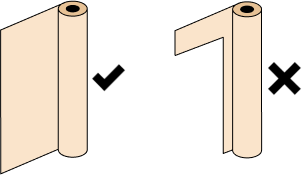
\includegraphics[width = \textwidth]{Images/bolt cutting.png}
    \caption{Cut from bolt assumption}
    \label{fig:cut from bolt}
\end{figure}

The efficiency computation are as follows:

cut loss width = ideal bolt width - pattern width \newline
cut loss area = cut loss width * pattern height \newline
efficiency = 100 * (1 - (cut loss area/ (pattern width * pattern height))

%%%%%%%%%%%%%%%%%%%%%%%%
% MITIGATION
%%%%%%%%%%%%%%%%%%%%%%%%

\subsection{Pattern Mitigation}
The default assumption is that the pattern width will fall along the bolt width (Figure \ref{fig:pw along bolt})
\begin{figure} [H]
    \centering 
    \includegraphics[width = 0.6\textwidth, angle=90]{Images/pw along bolt.png}
    \caption{Regular layout}
    \label{fig:pw along bolt}
\end{figure}

If the user prefers a fabric with a bolt width less than pattern width or if the ideal bolt width is unavailable, some mitigation is required. This will lead to added cut loss and potentially new seams. Complex, sophisticated fitting algoritms are beyong this project's scope. Instead, simple strategies to mitigate the cut loss are provided:

\subsubsection{Rotation}
If the bolt width is greater than pattern height, rotate the pattern 90º (Figure \ref{fig:ph along bolt}).
The waste then becomes:

Waste = (bolt width - pattern height) * pattern width
\begin{figure} [H]
    \centering
    \includegraphics[width = 0.8\textwidth]{Images/ph along bolt.png}
    \caption{Rotation layout}
    \label{fig:ph along bolt}
\end{figure}

\subsubsection{Symmetry}
If the bolt width is also less than pattern height, break the pattern into two symmetrical halves along the centre back line (Figure \ref{fig:symmetry split}). This will result in a sewn seam along the centre back in the finished garment and will need a ~1 cm seam allowance. So now each piece has a width equal to half the pattern width plus the seam allowance.

Resultant piece width = 0.5 * pattern width + seam allowance

The waste then becomes:

Waste = (bolt width - resultant piece width) * 2 * pattern height
\begin{figure} [H]
    \centering
    \includegraphics[width = 0.8\textwidth]{Images/symmetry split.png}
    \caption{Symmetry layout}
    \label{fig:symmetry split}
\end{figure}

\subsubsection{Breakout}
If even the previous resultant piece width is greater than the bolt width then break the pattern into four rectangles. Make a split between the bodice section (inclusive neck facings) and the combined sleeve and collar piece sections along and a split down the centre back line (Figure \ref{fig:breakout}). This has the potential for the most loss but is the tradeoff to use existing fabric from an avaliable smaller width bolt.
\begin{figure} [H]
    \centering
    \includegraphics[width = 0.6\textwidth, angle=90]{Images/break into 4.png}
    \caption{Breakout layout}
    \label{fig:breakout}
\end{figure}

%%%%%%%%%%%%%%%%%%%%%%%%
% EMBELLISHMENTS
%%%%%%%%%%%%%%%%%%%%%%%%

\subsubsection{Embellishments}
Even with a rectangular pattern based on the person's dimension, there is always the potential for cut loss. This is especially true if the `ideal bolt width' is not available. One way to recoup this cut loss is via embellishments.

Application of embellishments is highly dependent on the creativity of the fashion designer to generate extra utility by repurposing fabric. Embellishments just cannot be random pieces of fabric tacked onto the garment without a design purpose. For this garment type in this study, front chest pockets are a great embellishment that would well complement the shirt design. 

A standard finished pocket size is 10 cm by 10 cm. Front shirt pockets have sewing and hem allowances that typically are 0.5cm allowance for the sides and bottom edges and 2 cm hem allowance for the top edge to create a quality finish. Adding up these values for a finished pocket, we get a pocket pattern piece that is 11 cm by 12.5 cm. The cut loss width needs to be a minimum of 11 cm to fit the pocket. Smaller sizes, cut up and sewn together to get a finished pocket are not explored due to significantly increased complexity of construction.

This pocket embellishment is an example. The definition of the pocket is customisable. Any fashion designer / sewer can opt for a different size pocket / embellishment. For example a 8 cm by 8 cm finished pocket or a non square 8 cm by 10 cm finished pocket. Its size is not dependent on any body measurement. An example of a body measurement based embellishment is a belt. It would have different dimensions and construction requirements.

For analysis, we just need the dimensions of the embellishment. These are then checked against the cut loss dimension to see if recovery is possible and if so, then compute the percentage amount of the recovery. This analysis can be generalized to any embellishment at all. The only thing that needs to change is the instruction to the sewer on how to tailor this extra piece, of course alongside the new embellishment piece size to check for. An update to the DXF output allows this to be previewed in CLO 3D.

%%%%%%%%%%%%%%%%%%%%%%%%
% WORKSHOP STUDY
%%%%%%%%%%%%%%%%%%%%%%%%
\section{Workshop Study}

\subsection{Rationale}
The purpose of the workshop is to test out the garment pattern parameterisation process in the real world to see how it translates when working with physical material of the fabric. The report is focused on testing if the parameterisation process works well in creating a better fit for the individual while still keeping its intended style and aesthetic. The pattern is supposedly aimed at ‘confident beginners,’ and this author has tested it on their own. However, the efficacy of the pattern’s instruction needed to be verified in an observable setting. 

The research study workshop was part of a larger event that I led and organised for the Dyson Engineering Fashion and Textiles Research Group. The event allowed the research group folk to participate in the workshop and learn new skills like the use of the sewing machine, overlocker, and the tailoring process of going from bolt to finished garment.

\subsection{Methods}

\subsubsection{Experimental Procedures}
\noindent \textbf{Outreach}

A digital poster was made to advertise the workshop, shown in Appendix. The campaign was only advertised to the Dyson Engineering Fashion and Textiles Research Group who already have self described interest in the topic along with the skills needed to follow tailoring instruction. Participants were limited because of the time, resources, and expertise needed such as for example we only had 3 sewing machines.

\noindent \textbf{Clearances} 

Since personal data like body measurements were being gathered, participants’ consent as well as training in the ethical handling of the data were a prerequisite. Department ethics clearances were obtained by completing risk assessment training and filling the appropriate ethics forms. There was also an evaluation from the Events Risk Assessment team to obtain their approval for this activity.

All the participants were all given randomised unique alphanumeric identifiers, during the study to maintain anonymity. The participants only knew their data. For the purposes of the study the only requirement was to correctly identify and treat a group of measurements as belonging to one (unnamed) person.

Along with all the ethics and participant information sheet and informed consent forms, also created were pattern cutting and sewing instructions, the worksheet to follow along in the study/workshop, and paper patterns for an activity to understand the pattern.

\noindent \textbf{Process}

The workshop took place over 3 sessions:
\begin{enumerate}
    \item Initiation: Explaining the schedule and purpose of the study to the participants. Walkthrough of the process with the paper pattern activity, learning sewing basics, taking body measurements, and finally generating the bespoke patterns and working towards drawing and getting all pieces of the pattern cut out from the fabric.
    \item Sewing: Dedicated time towards sewing the garment from the given pattern.
    \item Evaluation: Finishing the garment and collecting metrics (both quantitative finished garment measurements and the qualitative perceptions of fit and comfort).
\end{enumerate}
Each of these sessions took about 4 hours each.

\noindent \textbf{Setup}

We had a total of eight participants, with six of them getting all the way through to the finished garment stage and fit evaluation.
\newline
The first step was to take body measurements. This was needed not only for the pattern creation but also for comparing the results of the fit and ease. This diagram and following instructions for measurement taking were provided so measurements were taken consistently.
\begin{figure} [H] % opens the figure environment. the '[H]' forces the image to be Here
    \centering % puts the image in the horizontal centre of the page
    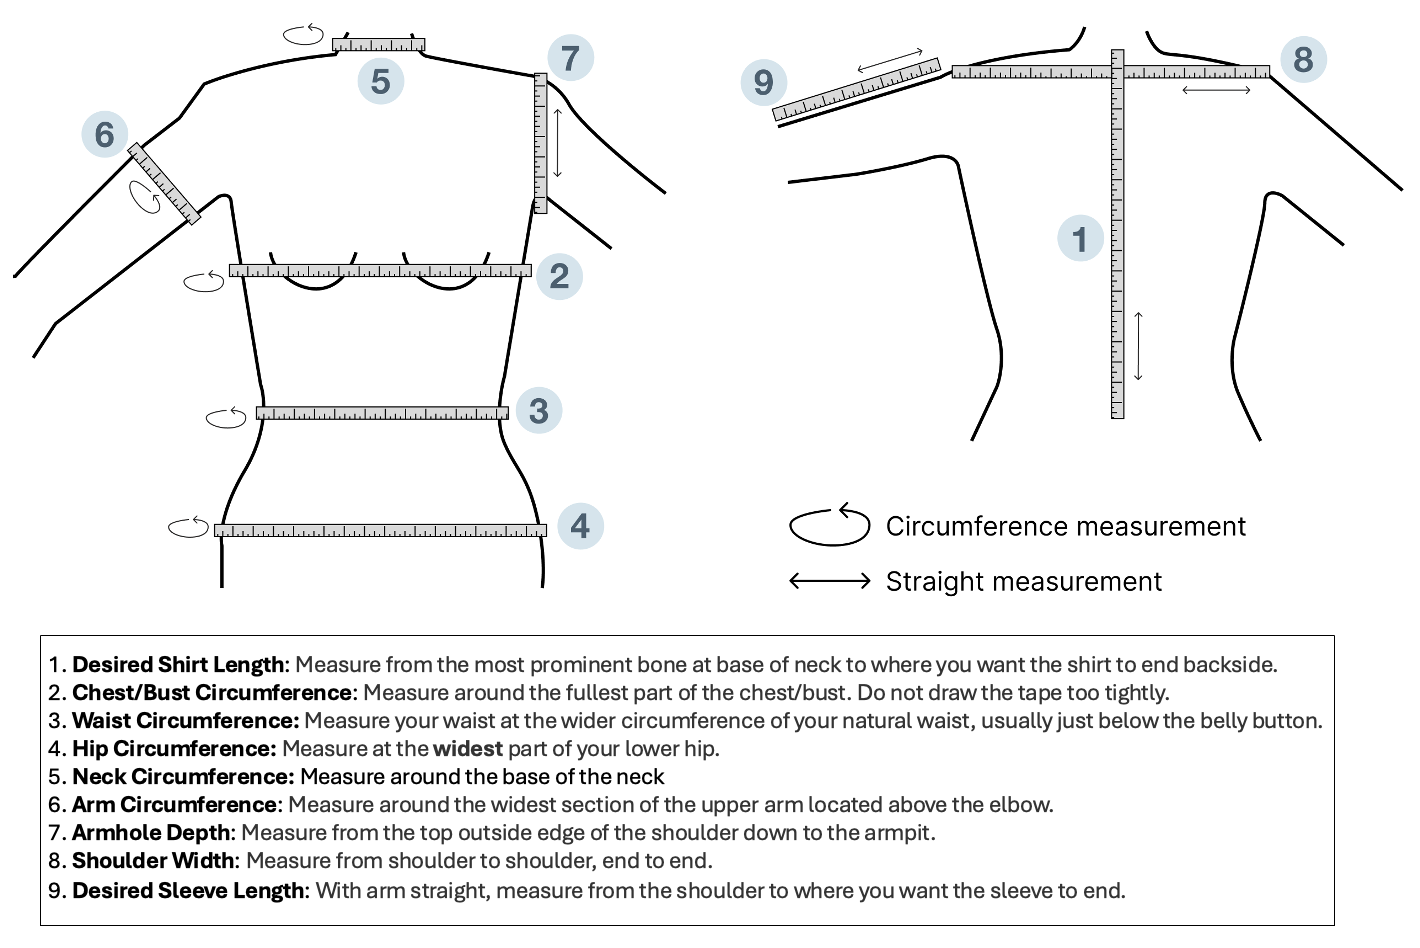
\includegraphics[width = \textwidth]{Images/workshopmeasure.png} %this tells latex what graphics to include. I put my images in an 'Images' folder to aid file management, hence the Images/ before the file name. the width bit before allows you to alter the width of the image. It is also possible to use scale as well as using equations with the textwidth to make it say half the text width.
    \caption{Workshop measurement taking instructions}
\end{figure}

% \begin{enumerate}
%     \item \textbf{Desired Shirt Length:} Measure from the most prominent bone at base of neck to where you want the shirt to end backside.
%     \item \textbf{Chest/Bust Circumference:} Measure around the fullest part of the chest/bust. Do not draw the tape too tightly.
%     \item \textbf{Waist Circumference:} Measure your waist at the wider circumference of your natural waist, usually just below the belly button.
%     \item \textbf{Hip Circumference:} Measure at the widest part of your lower hip.
%     \item \textbf{Neck Circumference:} Measure around the base of the neck
%     \item \textbf{Arm Circumference:} Measure around the widest section of the upper arm located above the elbow.
%     \item \textbf{Armhole Depth:} Measure from the top outside edge of the shoulder down to the armpit.
%     \item \textbf{Shoulder Width:} Measure from shoulder to shoulder, end to end.
%     \item \textbf{Desired Sleeve Length:} With arm straight, measure from the shoulder to where you want the sleeve to end (max 25 cm).
% \end{enumerate}
For the workshop the focus was on making toiles. A toile is "a prototype or fitting version of a garment that's made up in an inexpensive fabric so that the design can be tested and perfected". This was done to be efficient with time and get the most meaningful important results. Therefore, attention was paid to stitching the essential components like pleats, shoulders, and sleeves. The button placket and collar were less important and were just pinned on for fit evaluation if desired.

All participants were measured. Their individualised parameterized patterns were given to them along with an appropriately cut piece of fabric. They were then guided through the 3 sessions to make the garment. Once completed, measurements of the finished garment as well as the participants perception of fit and comfort were recorded. These will be used in evaluating the suitability of the parameterisation method.

%%%%%%%%%%%%%%%%%%%%%%%%
% 100 SCANS STUDY
%%%%%%%%%%%%%%%%%%%%%%%%
\section{Body Scans Study}

\subsection{Rationale}
The University of Manchester’s Apparel Design Engineering (ADE) team has made public 100 scans processed using a Size Stream body scanner. The scans are a sample of 20-30 year-old females from the UK, with half identified as White British and half as Chinese. This is known as the referred to as Mendeley dataset. From the dataset’s release notes, “3D Body Scanning is a technology that allows the capture and analysis of the human body using non-contact methods, current uses have allowed large datasets to be captured and comparisons made with population groups.”

This study needs to validate its processes across a larger dataset than was obtained in the workshop. The efficacy of modern 3D scanning technology also needs to be tested. The ADE data set satisfies both these criteria. In fact the data capture is more rigorous than found in a commercial tailoring setting. The precision and accuracy of the scanning technology far exceeds the data captured manually. The purpose of this study is focused around the fabric use efficiency metrics and efficacy of pattern mitigation strategies rather than fit analysis as these patterns will not be produced into physical garments.

\subsection{Methods}
The pattern parameterisation methods differ slightly because of the different approach to measurement taking that is carried out by the Size Stream scanner than that of manual measurement taking employed for the workshop. The Size Stream works by

I met with Simeon Gill to discuss and justify the measurements from the scan output that should be used this garment paramterisation. The Mendeley dataset provides many more datapoints and builds measurements from points defined on the body in its 3D space. For the circumference measurements around different areas of the body, the outputted data provides derivatives of the base/driving measurement (usually the circumference). The coding for these derivatives is as follows

c = circumference

TM = tape measure

f = front arc of the circ

b = back arc of the circ

d = depth of the circ

w = width of the circ

h = height of the circ

\textbf{(ADD DIAGRAMS FOR ALL OF THESE DERIVATIVES TO SHOW VISUAL EXAMPLES)}

Tape measure derivatives are useful for our patterns as these bridge concavities of the model as opposed to contours like the "c" coded measurement while closely follows the body surface. To determine the max bodice circumference, we analyse more than just the hip, waist, and chest/bust measurements. In fact, we take into considerations seven relevant bodice circumference TM measurements that reinforce inclusivity of body shapes: Abdomen Circ, Axilla Chest Circ, Chest/Bust Circ, Hip Circ, Seat Circ, Stomach Max Circ, Waist Circ. These are shown in the figures below. The parameterisation still takes the largest of these circumferences and adds the general ease and sew allowance to compute pattern 

\textbf{(ADD DIAGRAMS FOR ALL THESE CIRCS FROM THE SIZE STREAM OR RECREATE THEM IF NOT AVAILABLE)}

The height derivatives are measured from the floor straight up to specified point or arc in the Y plane. The heights of the circumferences are useful because they allow us to derive the relation to where various circumferences are to each other. For the ADE group focusing on more form fitting, non-zero waste clothing, this is useful because this will allow them to control ease around different parts of the body. They can produce a visual representation/estimation of where the body will take up space within the garment. An instance of this is shown in the below example of a bespoke sweatshirt pattern produced by the ADE group. 

For our purposes, the height derivatives will be useful in calculating the pattern height. Since the Mendeley dataset does not provide a center back base neck height and it is not applicable for the person to provide a desired shirt length, a new method for determining shirt length and thus pattern height consistently across all persons was devised.

To calculate the shirt length for the Mendeley scans the following measurements are used: Crotch Height, Waste Height, and Half Back Center TM. The Half Back Center TM extends from the the back neck landmark to the center back waist landmark measured along the contour of the back, seen in the image below. The back waist landmark is a point on the waist circumference so using the derivative waist height from it is appropriate. An important note is that the waist height and crotch height are straight lines and the half back center TM is a contour. Consultation with Simeon Gill decided that this will not affect the outcome greatly (being slightly longer shirt length than if the half back center measurment was a straight line) and is suitable for purposes of finding a consistent method of shirt length given we cannot get a desired input).
\begin{figure} [H] % opens the figure environment. the '[H]' forces the image to be Here
    \centering % puts the image in the horizontal centre of the page
    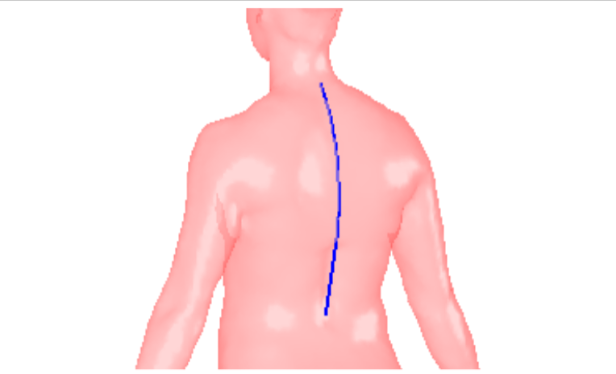
\includegraphics[width = 0.5\textwidth]{Images/HBC TM.png} %this tells latex what graphics to include. I put my images in an 'Images' folder to aid file management, hence the Images/ before the file name. the width bit before allows you to alter the width of the image. It is also possible to use scale as well as using equations with the textwidth to make it say half the text width.
    \caption{Half Back Center TM diagram}
\end{figure}
To calculate the shirt length, we will add the waist height to the half back center and substract the crotch height from it.

Shirt Length = Waist Height + Half Back Center TM - Crotch Height

This will be treated as the desired shirt length and plugged in to the pattern height formula as stated before in section 3.2. 

This data is run through the program to calculate the fabric use efficiencies and verify suitability of the pattern file construction.

\section{Personal Case Study}
I visited the ADE group in Manchester to get own scan data using the Size Stream scanner. The parameterisation for the pattern height and width differe slightly because of the slightly different data points provided. 
My data did not provide and Axilla Chest circumference so this was omitted when checking for max bodice circumference used in determining pattern width.

My data did not provide a half back center measurement but did provide the neck base circumference, unlike the Mendeley set. We will use the height derivative of the neck base circumference and subtract the crotch height from it to get my desired shirt length. Keeping the crotch height to have some consistency with the method used in 3.4.

Shirt Length = Neck Base Height - Crotch Height

A total of five scans of myself were taken. The median values for all measurements were used in the my pattern's parameterisation. Using the median values for creating the pattern is justified because the median is robust to outliers and better represents typical measurmeents in the presence of variability in body scan data could could arise from factors such as posture, breathing, and slight movements.

Unlike the Mendeley set, I also obtained the obj file of my scan. This 3D file can be imported into CLO and be used as an avatar. This is particularly useful to understand the virtual draping of the custom garment on the person it is intended for.

\textbf{ADD THE DIMENSION AND PATTERN FILE OUTPUTS FOR MY SCAN}

\textbf{ADD OBJ FILE IMPORT INTO CLO WITH MY GARMENT DRAPED ON}